%*******10********20********30********40********50********60********70********80

% For all chapters, use the newdefined chap{} instead of chapter{}
% This will make the text at the top-left of the page be the same as the chapter

\chap{How to Do}\label{chap:howtodo}
This is all I know on LaTex up to now.

\section{Including Sections and Subsections}
This is my first section.

\subsection{I like myself}
I'm nice.

\subsection{but I'm weird}
but fun.

\subsubsection{LOST OF FUN!}
Writing writing and writing.

\subsubsection{I'm calm and shit}
I write stuff in subsubsections.

\paragraph*{And lastly this is new and amazing PARAGRAPH:} You can write whatever you want and it's pretty cool and new. I still like subsubsections more. 

\section{Including references and citations}
This is pretty simple to cite: developed as open-source C++ software by Rudolf Biczok \cite{paraunity}.
We'll learn more about this as we go.

%Funny stuff about myself \parencite[see][]{7.4article}.
%Let's see what cite command \cite[see][]{8article} does.

%Relax \parencite[see][p10]{nelson}
%This is a reference \parencite[see][]{7.1article}

\subsection{Referencing images and tables!}
So you can see figure \ref{fig:living} at page \pageref{living}. AMAZING\\
OR you can also see the table \ref{tab:temps} at page \pageref{tab:temps}!

\subsection{Referencing chapters and subchapters}
You can also ref chapters, as Chapter Results \ref{chap:results}.

\subsection{Using footnotes}
Let's try this out.\footnote{This is my first footnote.} And another one to see if it is progressive and shit.\footnote{CAREFUL! Don't leave any spaces before the command or they will be rendered.}\\

I'll try now to ''place them manually''. This is were the sign is.\footnotemark \\
Somewhere else in the text. I insert what it contains.\footnotetext{This is my footnote!}

\section{Including quotes}
This is how a quote looks. 

\begin{displayquote}
	From an evolutionary perspective, virtual reality is seen as a way to overcome limitations of standard human-computer interfaces; from a revolutionary perspective, virtual reality technology opens the door to new types of applications that exploit the possibilities offered by presence simulation.
\end{displayquote}

And also in text quotes: \enquote{[by] immersing the user in the solution, virtual reality reveals the spatially complex structures in computational science in a way that makes them easy to understand and study}.

And dots\dots

\section{Including code}
The following code is written by Lorenzo:

% Code from Lorenz
%\begin{minipage}{\linewidth}
%\begin{lstlisting}
%	public void ToggleShow(bool show) {
%		// Hide all walls
%		foreach (GameObject wall in walls)
%			wall.SetActive(show);
%			
%		// Set default material to floor
%		floor.SetMaterial(show);
%	}
%\end{lstlisting}
%\end{minipage}

% Code from me
\begin{minipage}{\linewidth}
\begin{lstlisting}
=IF(
   OR(
      E68 = "Russia";
      E68 = "Albania";
      E68 = "Bulgaria";
      E68 = "Ungheria";
      E68 = "Ucraina";
      E68 = "Moldavia";
      E68 = "Romania"
   );
   "Europa dell'Est";
   IF(
      OR(
         E68 = "Burkina Faso";
         E68 = "Etiopia";
         E68 = "Costa d'Avorio";
         E68 = "Congo";
         E68 = "Guinea Bissau";
         E68 = "Africa";
         E68 = "Ghana";
         E68 = "Benin"
      );
      "Africa";
      IF(
         OR(
            E68 = "Colombia";
            E68 = "Brasile";
            E68 = "Guatemala";
            E68 = "Peru";
            E68 = "Costa Rica"
         );
         "America del Sud";
         IF(
            OR(
               E68 = "Armenia";
               E68 = "India";
               E68 = "Cina";
               E68 = "Vietnam";
               E68 = "Sri Lanka";
               E68 = "Siberia";
               E68 = "Nepal";
               E68 = "Filippine"
            );
            "Asia";
            ""
         )
      )
   )
)
\end{lstlisting}
\end{minipage}

\section{Formatting Text}
\textbf{This is BOLD}
\textit{This is ITALIC}
\textsf{This is SANS SERIF}
\texttt{This is TRUE TYPE}

In this sentence {\tiny{THIS IS TINY}}.
\tiny THIS WHOLE SENCE IS TINY.

\normalsize I go back to normal.

Then I can go for {\large{large}}, or {\Large{Large}}, or {\LARGE{Larger}}, or {\huge{Huge}} and even {\Huge{HUGE}}.

\section{Including bulleted list}
Lorem ipsum dolor sit amet, consectetur adipiscing elit. Nam quam tellus, venenatis a consectetur non, pretium ac nunc. Nullam eu tellus sed augue laoreet scelerisque. 

\begin{itemize}
    \item The first item of your list
    \item The second item of your list
    \item The third item of your list
\end{itemize}

Lorem ipsum dolor sit amet, consectetur adipiscing elit. Nam quam tellus, venenatis a consectetur non, pretium ac nunc. Nullam eu tellus sed augue laoreet scelerisque. Curabitur efficitur, dolor ut pretium fermentum, nisi enim pulvinar nunc, non bibendum urna odio nec neque. Cras tellus turpis, posuere in dictum vitae, vestibulum quis velit.

\begin{enumerate}
    \item The first item of your list
    \item The second item of your list
    \item The third item of your list
\end{enumerate}

Lorem ipsum dolor sit amet, consectetur adipiscing elit. Nam quam tellus, venenatis a consectetur non, pretium ac nunc. Nullam eu tellus sed augue laoreet scelerisque. Curabitur efficitur, dolor ut pretium fermentum, nisi enim pulvinar nunc, non bibendum urna odio nec neque. Cras tellus turpis, posuere in dictum vitae, vestibulum quis velit. 

\begin{description}
    \item[a)] The first item of your list
    \item[b)] The second item of your list
    \item[c)] The third item of your list
\end{description}
 

\section{Including Figures}
Orci varius natoque penatibus et magnis dis parturient montes, nascetur ridiculus mus. Nam vulputate finibus malesuada. Praesent at egestas turpis. Vivamus vitae tellus malesuada, laoreet ex ac, venenatis est. Aliquam dictum tincidunt libero, cursus posuere arcu sodales non. In sed metus sit amet arcu vestibulum mollis ut vel nibh. Nam non velit tortor. Integer ac sapien a purus porta convallis. In vestibulum aliquam nunc vitae faucibus. Etiam tristique iaculis orci, vel aliquam felis accumsan et. Nulla ultricies, nisl eu malesuada lobortis, ante metus faucibus libero, vitae blandit odio enim sit amet tortor.

% Living room
\begin{figure}[ht]
	\centering
	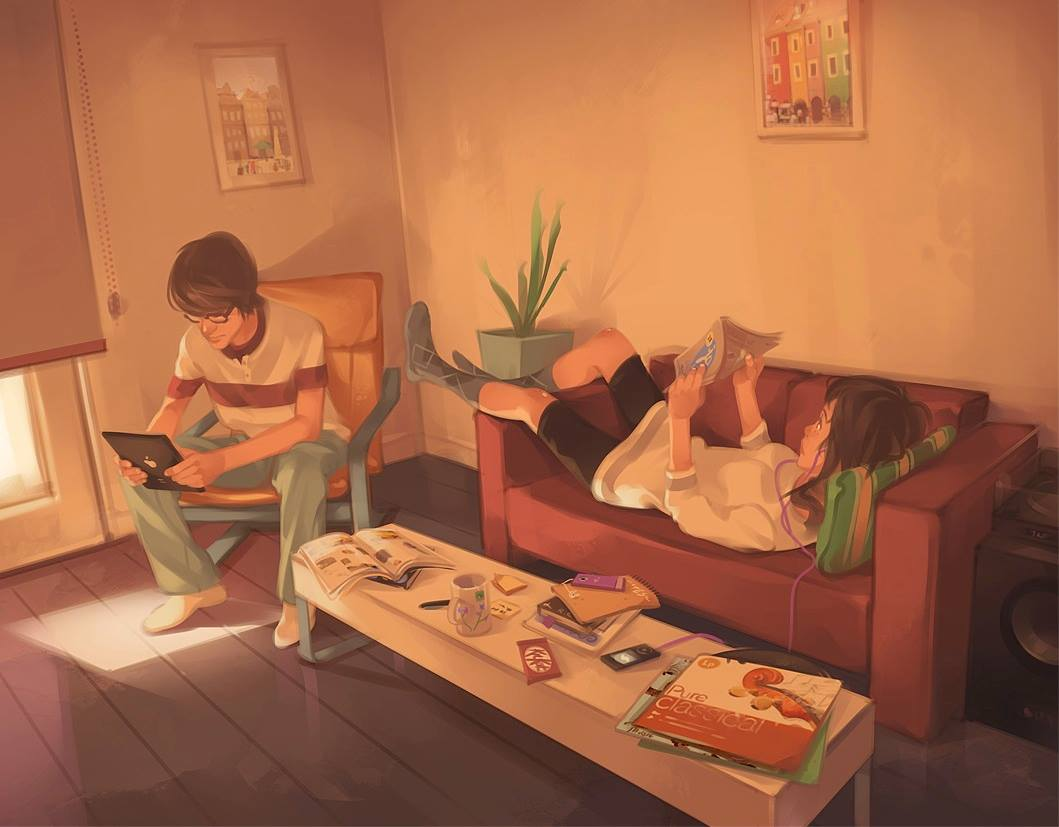
\includegraphics[width=\textwidth]{living}
	\caption{Living room as I imagine it}
	\source{Photo courtesy of HTC}
	\label{fig:living}
\end{figure}

\section{Including Tables}
Orci varius natoque penatibus et magnis dis parturient montes, nascetur ridiculus mus. Nam vulputate finibus malesuada. Praesent at egestas turpis. Vivamus vitae tellus malesuada, laoreet ex ac, venenatis est. Aliquam dictum tincidunt libero, cursus posuere arcu sodales non. In sed metus sit amet arcu vestibulum mollis ut vel nibh. Nam non velit tortor. Integer ac sapien a purus porta convallis. In vestibulum aliquam nunc vitae faucibus. Etiam tristique iaculis orci, vel aliquam felis accumsan et. Nulla ultricies, nisl eu malesuada lobortis, ante metus faucibus libero, vitae blandit odio enim sit amet tortor.

\begin{table}[ht!]
    \begin{subtable}[h]{0.45\textwidth}
        \centering
        \begin{tabular}{l | l | l}
        Day & Max Temp & Min Temp \\
        \hline \hline
        Mon & 20 & 13\\
        Tue & 22 & 14\\
        Wed & 23 & 12\\
        Thurs & 25 & 13\\
        Fri & 18 & 7\\
        Sat & 15 & 13\\
        Sun & 20 & 13
        \end{tabular}
        \caption{First Week}
        \label{tab:week1}
    \end{subtable}
    \hfill
    \begin{subtable}[h]{0.45\textwidth}
        \centering
        \begin{tabular}{l | l | l}
        Day & Max Temp & Min Temp \\
        \hline \hline
        Mon & 17 & 11\\
        Tue & 16 & 10\\
        Wed & 14 & 8\\
        Thurs & 12 & 5\\
        Fri & 15 & 7\\
        Sat & 16 & 12\\
        Sun & 15 & 9
        \end{tabular}
        \caption{Second Week}
        \label{tab:week2}
    \end{subtable}
    \caption{Max and min temps recorded in the first two weeks of July}
    \label{tab:temps}
\end{table}

% Paraview Architecture
\begin{table}[ht] 
	\centering 
	\def\arraystretch{1.5}
	\begin{tabular}{|c|c|c|c|}
		\hline
		\rowcolor{tblpink}
		\multicolumn{4}{|c|}{\textbf{ParaView}} \\
		\hline
		\rowcolor{tblorange}
		\multicolumn{4}{|c|}{\textbf{VTK}} \\
		\hline
		\rowcolor{tblgreen}
		\textbf{OpenGL} & \textbf{MPI} & \textbf{OpenVR} & \textbf{Etc.} \\
		\hline
	\end{tabular}
	\captionof{table}{ParaView-VTK Architecture (simplified)}
	\label{tab:paraviewArchitecture}
\end{table}